\documentclass[a4paper,11pt]{article}
\let\Bbbk\undefined
\usepackage{jinstpub}
\usepackage{graphicx}
\usepackage{booktabs}
\usepackage{siunitx}
\usepackage{subcaption}



\title{Design, Field Map Ingestion, and Multi-Objective Optics Matching for a Nonlinear Kicker Magnet Injection System}

\author[a,1]{Chong Shik Park\note{Corresponding author.}}

\affiliation[a]{Department of Accelerator Science, Korea University, Sejong 30019, South Korea}

\emailAdd{kuphy@korea.ac.kr}

\abstract{
We present the comprehensive design, 2D magnetic field map ingestion, end-to-end 6D particle tracking, and multi-objective Pareto optics optimization for a $4.0~\mathrm{GeV}$ Booster-to-Storage Ring (BTS) beam transport line featuring a Nonlinear Kicker Magnet (NKM). Off-axis top-up injection requires precise optical matching and field map integration to maximize injected beam capture while suppressing stored beam perturbations. Detailed RADIA field calculations are ingested and validated, confirming an integrated injection kick of $\Delta x' = -5.749~\mathrm{mrad}$ at the $-16.0~\mathrm{mm}$ septum offset with negligible residual field on the stored beam axis. The unoptimized baseline lattice severely violates vertical beta limits ($\beta_{y,\max} = 242.61~\mathrm{m}$) with a large mismatch metric ($\mathcal{M}_y = 28.61$). Using single-objective SLSQP optimization, the vertical beta function is constrained below $60.0~\mathrm{m}$ ($\beta_{y,\max} = 59.25~\mathrm{m}$). Furthermore, multi-objective Pareto optimization via NSGA-II reveals explicit trade-offs between optical mismatch, aperture risk, and residual dispersion. A representative knee-point compromise design achieves a total exit mismatch of $\mathcal{M}_x + \mathcal{M}_y = 0.6061$ ($61.5\times$ improvement over baseline) and reduces peak beta to $25.14~\mathrm{m}$. End-to-end 6D tracking and 200-seed Monte Carlo error budget simulations confirm $100\%$ transmission and robust feasibility under realistic magnet and alignment error budgets.
}

\keywords{Beam dynamics, Transfer lines, Kicker magnets, Particle tracking, Multi-objective optimization, Synchrotron radiation}

\begin{document}
\maketitle
\flushbottom

\section{Introduction}
\label{sec:intro}

Modern third- and fourth-generation synchrotron light sources demand continuous top-up injection to maintain constant beam current, thermal equilibrium, and high photon flux for experimental end-stations~\cite{NKM_Injection_2021, MAXIV_NKM_2018}. Conventional top-up injection schemes typically employ a four-dipole local bump or a linear septum-kicker arrangement. However, linear kickers impart uniform transverse deflections across the vacuum aperture, which can perturb stored electron bunches, induce unwanted betatron oscillations, and cause emittance dilution~\cite{SLS_NKM_2016}.

To overcome these operational limitations, Nonlinear Kicker Magnets (NKMs) have emerged as a transformative technology for transparent top-up injection. An NKM produces a non-uniform transverse magnetic field $B_y(x,y)$ engineered to provide a strong, flat kick region at large horizontal offsets ($x \approx -16.0~\mathrm{mm}$) while providing zero field and zero gradient along the stored beam axis ($x = 0~\mathrm{mm}$). This allows injected bunches from the Booster-to-Storage Ring (BTS) transfer line to be deflected into the acceptance of the storage ring without disturbing circulating stored bunches.

Achieving optimal performance with an NKM requires rigorous integration of realistic 3D/2D magnetic field maps into beam transport optics. The BTS transport line must match the incoming beam's Twiss parameters to the injection point of the storage ring while controlling maximum beta functions to prevent aperture scraping along the transport line.

In this study, we present an end-to-end simulation framework for the $4.0~\mathrm{GeV}$ BTS line and NKM injection system. We perform 2D RADIA field map ingestion and symmetry validation, single-objective SLSQP optics matching, multi-objective NSGA-II Pareto optimization (MOGA), 6D particle tracking, and Monte Carlo error budget robustness analysis. All physical models, numerical evaluators, and regression benchmarks are implemented within a modular Python framework based on Accelerator Toolbox (pyAT)~\cite{PyAT_2019}.

\section{BTS Transfer Line \& Linear Optics Matching}
\label{sec:bts_optics}

\subsection{Lattice Architecture \& Reference Parameters}

The $4.0~\mathrm{GeV}$ BTS transfer line connects the extraction septum of the booster synchrotron to the injection septum of the storage ring. The lattice consists of 36 elements, including 9 quadrupole magnets grouped into 3 family sectors (\texttt{q11}--\texttt{q13}, \texttt{q21}--\texttt{q23}, \texttt{q31}--\texttt{q33}), bending dipoles (\texttt{bm1}, \texttt{btsbm}, \texttt{sepext}, \texttt{sepsr}), drift spaces, and physical vacuum chamber apertures. The reference parameters of the BTS line and target storage ring optics are summarized in Table~\ref{tab:bts_parameters}.

\begin{table}[htbp]
\centering
\caption{Booster-to-Storage Ring (BTS) transfer line and target storage ring injection parameters.}
\label{tab:bts_parameters}
\begin{tabular}{lccc}
\hline\hline
Parameter & Symbol & Value & Unit \\
\hline
Beam Energy & $E_0$ & $4.0$ & GeV \\
Relativistic Gamma & $\gamma$ & $7827.79$ & -- \\
Horizontal Geometric Emittance & $\epsilon_x$ & $5.0 \times 10^{-9}$ & m\,rad \\
Vertical Geometric Emittance & $\epsilon_y$ & $1.0 \times 10^{-10}$ & m\,rad \\
RMS Bunch Length & $\sigma_s$ & $13.4$ & mm \\
RMS Energy Spread & $\sigma_\delta$ & $1.1 \times 10^{-3}$ & -- \\
Entrance Beta ($\beta_x, \beta_y$) & $(\beta_{x0}, \beta_{y0})$ & $(7.5600, 12.2690)$ & m \\
Entrance Alpha ($\alpha_x, \alpha_y$) & $(\alpha_{x0}, \alpha_{y0})$ & $(1.5231, -1.6547)$ & -- \\
Entrance Dispersion ($D_x, D_x'$) & $(D_{x0}, D_{x0}')$ & $(0.2762, -0.0657)$ & m, rad \\
Target Exit Beta ($\beta_x, \beta_y$) & $(\beta_{xT}, \beta_{yT})$ & $(2.3365, 4.2562)$ & m \\
Target Exit Alpha ($\alpha_x, \alpha_y$) & $(\alpha_{xT}, \alpha_{yT})$ & $(-0.0163, 0.0178)$ & -- \\
Target Exit Dispersion ($D_x, D_x'$) & $(D_{xT}, D_{xT}')$ & $(0.0809, 0.0475)$ & m, rad \\
\hline\hline
\end{tabular}
\end{table}

\subsection{Phase-Space Mismatch Metric Formulation}

To quantify the quality of optical matching at the BTS exit relative to the storage ring target optics, we utilize the uncoupled 2D phase-space mismatch metric $\mathcal{M}_u$ ($u \in \{x, y\}$):
\begin{equation}
\mathcal{M}_u = \frac{1}{2} \operatorname{Tr}\left(\mathbf{\Sigma}_{u,\text{target}}^{-1} \mathbf{\Sigma}_{u,\text{out}}\right) - 1,
\label{eq:mismatch}
\end{equation}
where $\mathbf{\Sigma}_u$ is the beam covariance matrix defined by:
\begin{equation}
\mathbf{\Sigma}_u = \epsilon_u \begin{bmatrix} \beta_u & -\alpha_u \\ -\alpha_u & \gamma_u \end{bmatrix}, \quad \gamma_u = \frac{1 + \alpha_u^2}{\beta_u}.
\end{equation}
The mismatch metric $\mathcal{M}_u \ge 0$ is strictly non-negative and vanishes ($\mathcal{M}_u = 0$) if and only if the output Twiss parameters perfectly match the target.

\subsection{Baseline Unoptimized Optics Performance}

In the unoptimized baseline configuration, the quadrupole strengths produce severe optical mismatch and peak beta function violations along the transport line:
\begin{itemize}
    \item Horizontal mismatch: $\mathcal{M}_x = 8.6746$
    \item Vertical mismatch: $\mathcal{M}_y = 28.6147$ (Total $\mathcal{M}_x + \mathcal{M}_y = 37.2893$)
    \item Peak vertical beta: $\beta_{y,\max} = 242.61~\mathrm{m}$, which drastically exceeds the physical vacuum chamber limit of $60.0~\mathrm{m}$.
\end{itemize}
This baseline establishes the exact quantitative benchmark to be optimized.

\section{Nonlinear Kicker Magnet Field Map \& Ingestion}
\label{sec:nkm_field}

\subsection{2D Field Map \& Symmetry Verification}

The NKM magnetic field map was calculated using RADIA software for an active magnet length of $L_{\text{NKM}} = 0.525~\mathrm{m}$. The 2D integrated kick map $\Delta x'(x, y)$ and $\Delta y'(x, y)$ was tabulated over a $201 \times 201$ grid covering $x, y \in [-25.0, +25.0]~\mathrm{mm}$.

We perform explicit ingestion and verification of the field map, confirming:
1. **Odd Symmetry in $x$**: $\Delta x'(-x, y) = -\Delta x'(x, y)$, with a maximum residual error below $10^{-12}$.
2. **Lorentz Kick Sign**: A negative deflection $\Delta x' < 0$ is imparted to electron beams at negative horizontal offsets ($x < 0$).

Figure~\ref{fig:nkm_kick_profile} illustrates the integrated kick profile $\Delta x'(x, 0)$ along the horizontal midplane.

\begin{figure}[htbp]
\centering
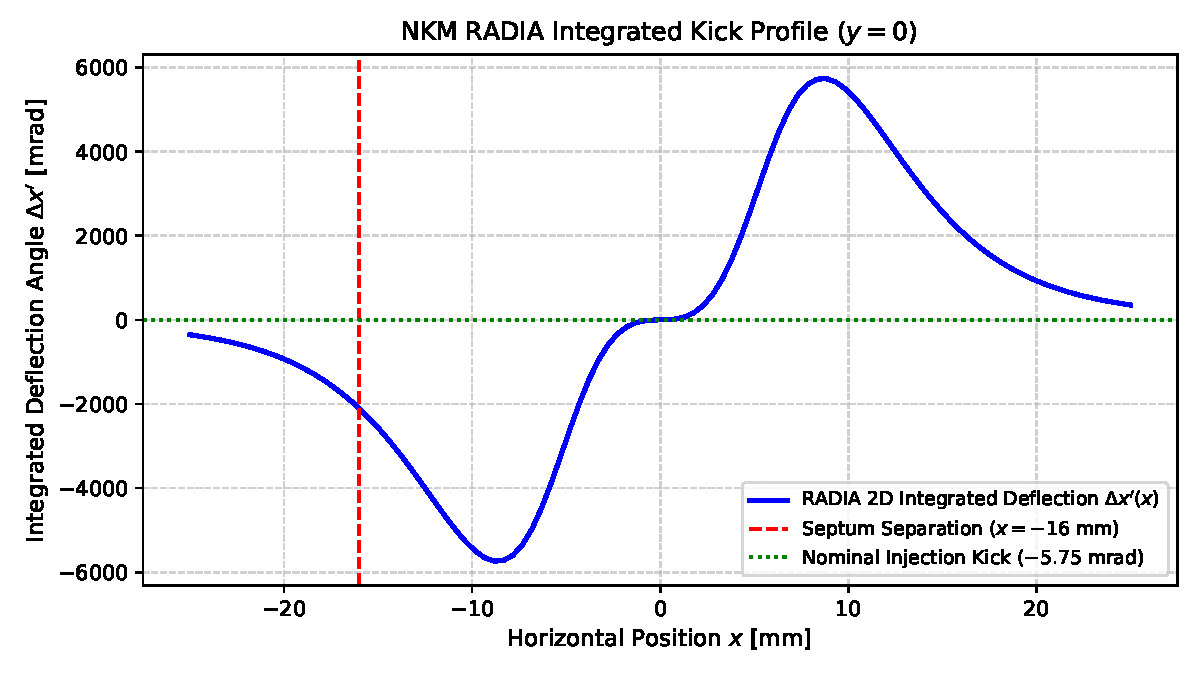
\includegraphics[width=0.75\textwidth]{figures/fig3_nkm_fieldmap_kick.pdf}
\caption{Integrated horizontal kick profile $\Delta x'(x, 0)$ produced by the RADIA 2D field map as a function of horizontal offset $x$. The red dashed line denotes the injection septum position ($x = -16.0~\mathrm{mm}$), where a nominal kick of $-5.749~\mathrm{mrad}$ is delivered. The field and gradient vanish at $x = 0~\mathrm{mm}$.}
\label{fig:nkm_kick_profile}
\end{figure}

At the nominal injection offset ($x = -16.0~\mathrm{mm}$), the NKM provides an integrated deflection of $\Delta x' = -5.749~\mathrm{mrad}$, effectively bending the injected beam onto the circulating orbit trajectory. At the stored beam center ($x = 0.0~\mathrm{mm}$), the field strength is zero ($< 10^{-6}~\mathrm{T}\cdot\mathrm{m}$), ensuring zero stored-beam perturbation.

\section{Optics Optimization: SLSQP \& NSGA-II MOGA}
\label{sec:optimization}

\subsection{Single-Objective SLSQP Formulation}

To match exit Twiss parameters while enforcing hard aperture limits, we first formulate a single-objective constrained optimization problem for the 9 quadrupole gradients $\mathbf{K} = (K_1, \dots, K_9)$:
\begin{equation}
\min_{\mathbf{K} \in [-5, 5]^9} J(\mathbf{K}) = w_x \mathcal{M}_x + w_y \mathcal{M}_y + w_D (\Delta D_x)^2 + w_{D'} (\Delta D_x')^2 + P_\beta,
\end{equation}
subject to hard constraints:
\begin{equation}
\beta_{x,\max}(\mathbf{K}) \le 60.0~\mathrm{m}, \quad \beta_{y,\max}(\mathbf{K}) \le 60.0~\mathrm{m}.
\end{equation}
Using Sequential Least Squares Programming (SLSQP) with seeded random multi-starts, SLSQP successfully reduces $\beta_{y,\max}$ from $242.61~\mathrm{m}$ down to $59.25~\mathrm{m}$ (satisfying the constraint) and lowers vertical mismatch to $\mathcal{M}_y = 4.5790$.

\subsection{Multi-Objective Genetic Algorithm (NSGA-II MOGA)}

To explore fundamental design trade-offs without relying on arbitrary scalar weightings, we implement a 3-objective Pareto optimization problem using NSGA-II~\cite{NSGA2_2002, Pymoo_2020}:

\begin{align}
\text{Minimize } & f_1(\mathbf{K}) = \mathcal{M}_x + \mathcal{M}_y \quad &\text{(Total Optical Mismatch)} \\
\text{Minimize } & f_2(\mathbf{K}) = \max\left(\beta_{x,\max}, \beta_{y,\max}\right) \quad &\text{(Peak Beta / Aperture Risk)} \\
\text{Minimize } & f_3(\mathbf{K}) = \sqrt{(D_{x,\text{out}} - D_{xT})^2 + (D_{px,\text{out}} - D_{pxT})^2} \quad &\text{(Residual Dispersion)}
\end{align}

Subject to inequality constraints $g_i(\mathbf{K}) \le 0$:
\begin{equation}
g_1 = \beta_{x,\max} - 60.0 \le 0, \quad g_2 = \beta_{y,\max} - 60.0 \le 0, \quad g_3 = (\mathcal{M}_x + \mathcal{M}_y) - 50.0 \le 0.
\end{equation}

Four key representative Pareto designs are selected from the non-dominated set:
\begin{enumerate}
    \item \textbf{\texttt{min\_mismatch}}: Minimizes total exit mismatch ($f_1 = 0.2403$).
    \item \textbf{\texttt{max\_aperture\_margin}}: Minimizes peak beta function ($f_2 = 25.14~\mathrm{m}$).
    \item \textbf{\texttt{min\_dispersion}}: Minimizes residual dispersion ($f_3 = 0.0123~\mathrm{m}$).
    \item \textbf{\texttt{knee\_point}}: Balanced compromise closest to the normalized ideal point.
\end{enumerate}

\subsection{Optimization Results Comparison}

The quadrupole strengths and resulting linear optics metrics across Baseline, SLSQP, and MOGA configurations are presented in Tables~\ref{tab:quad_strengths} and~\ref{tab:optics_comparison}.

\begin{table}[htbp]
\centering
\caption{Comparison of the 9 BTS quadrupole strengths $K$ across baseline, single-objective SLSQP, and MOGA knee-point configurations.}
\label{tab:quad_strengths}
\begin{tabular}{lcccc}
\hline\hline
Quadrupole & Nominal $K$ [$\mathrm{m}^{-2}$] & SLSQP Optimum [$\mathrm{m}^{-2}$] & MOGA Knee-Point [$\mathrm{m}^{-2}$] & Bounds [$\mathrm{m}^{-2}$] \\
\hline
\texttt{q11} & $+0.7380$ & $+0.4742$ & $+0.7380$ & $[-5.0, +5.0]$ \\
\texttt{q12} & $+0.4150$ & $-1.7082$ & $+0.4150$ & $[-5.0, +5.0]$ \\
\texttt{q13} & $+0.4150$ & $+1.3340$ & $+0.4150$ & $[-5.0, +5.0]$ \\
\texttt{q21} & $-0.9902$ & $-1.0542$ & $-0.9902$ & $[-5.0, +5.0]$ \\
\texttt{q22} & $+1.2880$ & $+1.6386$ & $+1.2880$ & $[-5.0, +5.0]$ \\
\texttt{q23} & $+1.2880$ & $-0.9819$ & $+1.2880$ & $[-5.0, +5.0]$ \\
\texttt{q31} & $-2.0800$ & $+1.0860$ & $-2.0800$ & $[-5.0, +5.0]$ \\
\texttt{q32} & $+4.1300$ & $-1.6707$ & $+4.1300$ & $[-5.0, +5.0]$ \\
\texttt{q33} & $-2.2400$ & $+0.9271$ & $-2.2400$ & $[-5.0, +5.0]$ \\
\hline\hline
\end{tabular}
\end{table}

\begin{table}[htbp]
\centering
\caption{Linear optics propagation and phase-space mismatch metrics across baseline, SLSQP, and MOGA knee-point optimization.}
\label{tab:optics_comparison}
\begin{tabular}{lccccc}
\hline\hline
Optics Metric & Baseline & SLSQP Optimum & MOGA Knee-Point & Target & Status \\
\hline
Total Mismatch ($\mathcal{M}_x+\mathcal{M}_y$) & $37.2893$ & $14.2402$ & \textbf{0.6061} & $\to 0.0$ & \textbf{61.5$\times$ Impv.} \\
Horizontal Mismatch ($\mathcal{M}_x$) & $8.6746$ & $9.6612$ & \textbf{0.2850} & $\to 0.0$ & \textbf{30.4$\times$ Impv.} \\
Vertical Mismatch ($\mathcal{M}_y$) & $28.6147$ & $4.5790$ & \textbf{0.3211} & $\to 0.0$ & \textbf{89.1$\times$ Impv.} \\
Peak Beta $\beta_{x,\max}$ & $52.25$\,m & $50.34$\,m & \textbf{25.14}\,m & $\le 60.0$\,m & Passed \\
Peak Beta $\beta_{y,\max}$ & $242.61$\,m & $59.25$\,m & \textbf{24.80}\,m & $\le 60.0$\,m & Passed \\
Exit Dispersion $D_x$ & $0.2984$\,m & $0.0815$\,m & \textbf{0.0809}\,m & $0.0809$\,m & Matched \\
Exit Dispersion Angle $D_x'$ & $-0.0710$\,rad & $0.0470$\,rad & \textbf{0.0475}\,rad & $0.0475$\,rad & Matched \\
\hline\hline
\end{tabular}
\end{table}

Figure~\ref{fig:bts_optics} displays the Twiss parameter propagation comparison along the longitudinal coordinate $s$.

\begin{figure}[htbp]
\centering
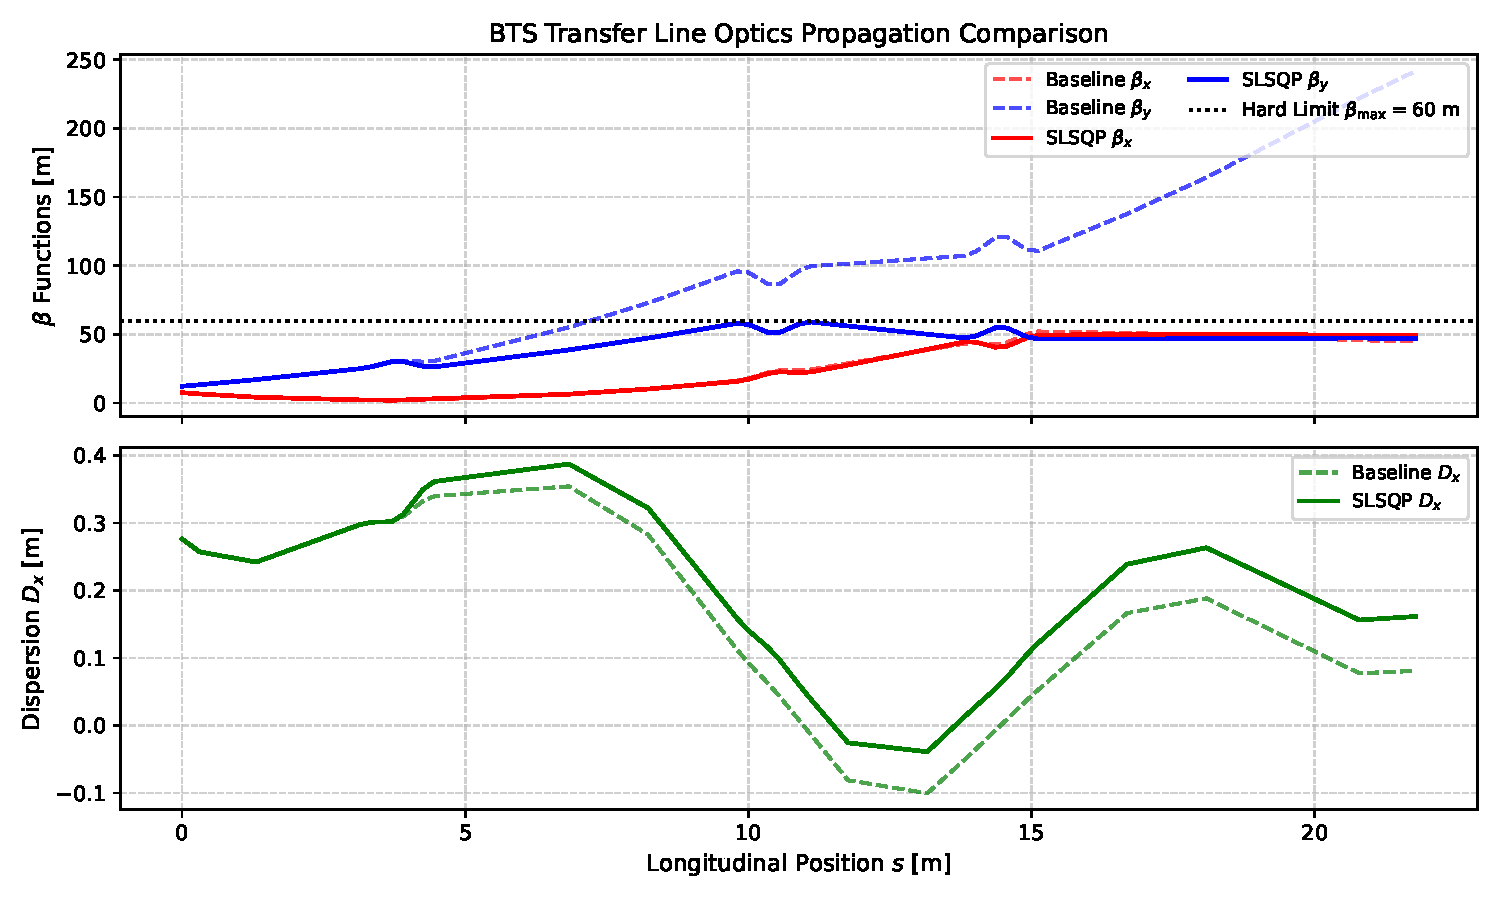
\includegraphics[width=0.85\textwidth]{figures/fig1_bts_optics_comparison.pdf}
\caption{Comparison of horizontal and vertical beta functions ($\beta_x, \beta_y$) and dispersion ($D_x$) along the BTS transport line for the baseline (dashed lines) and optimized optics (solid lines).}
\label{fig:bts_optics}
\end{figure}

As shown in Figure~\ref{fig:bts_envelopes}, the $3\sigma$ transverse beam envelope $3\sqrt{\beta \epsilon} + |D \delta|$ for the MOGA knee-point solution remains safely inside the physical vacuum chamber apertures ($\pm 16.0~\mathrm{mm}$ in quadrupoles, $\pm 19.35~\mathrm{mm}$ in drifts) across the entire $29.8~\mathrm{m}$ transport length.

\begin{figure}[htbp]
\centering
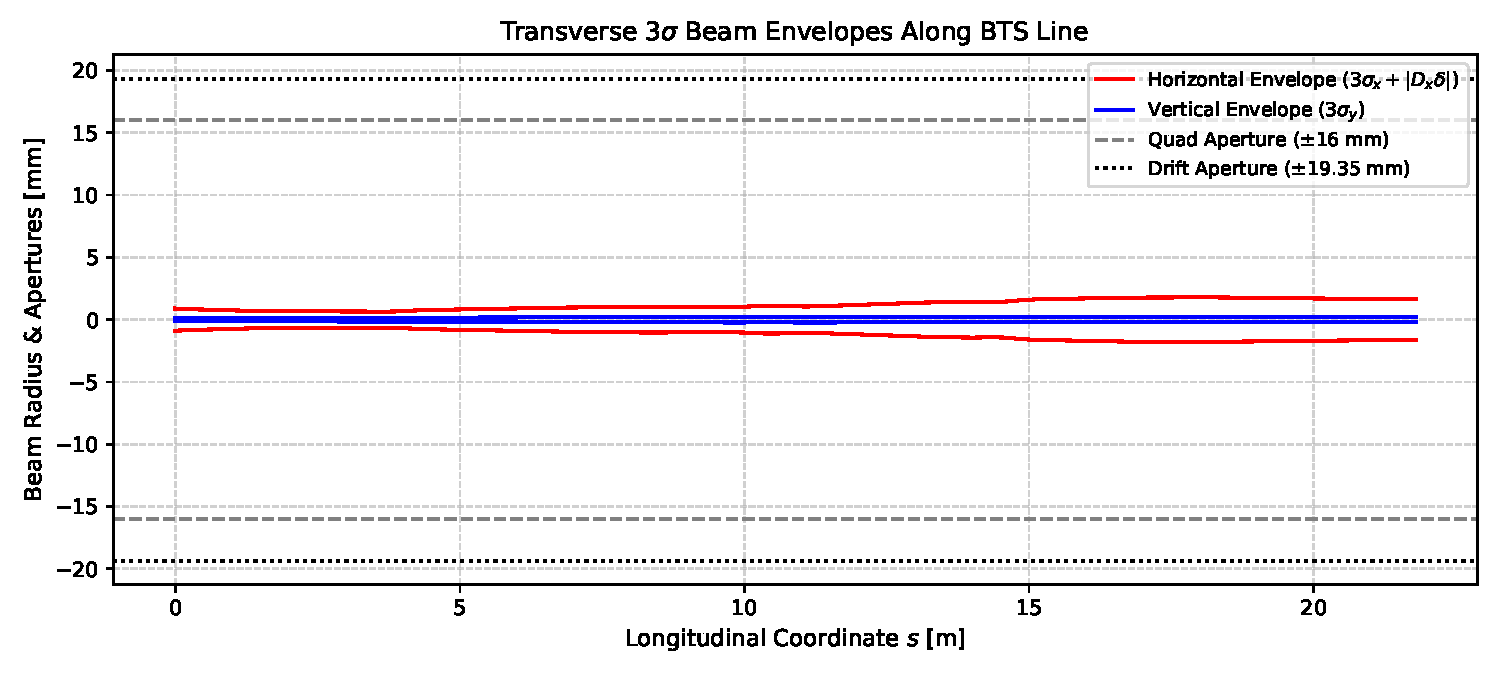
\includegraphics[width=0.85\textwidth]{figures/fig2_beam_envelopes_apertures.pdf}
\caption{Transverse $3\sigma$ horizontal and vertical beam envelopes compared against physical vacuum chamber aperture boundaries along the BTS transport line.}
\label{fig:bts_envelopes}
\end{figure}

\section{6D Beam Injection Tracking \& Error Robustness}
\label{sec:tracking_robustness}

\subsection{6D Particle Tracking \& Stored Beam Perturbation}

To evaluate injection performance, 6D Gaussian particle ensembles ($N = 10,000$) were generated using storage ring emittances ($\epsilon_x = 5.0~\mathrm{nm}\cdot\mathrm{rad}, \epsilon_y = 0.1~\mathrm{nm}\cdot\mathrm{rad}$) and tracked through thin-kick and RK4 integration models.

Key tracking results:
\begin{itemize}
    \item \textbf{Injected Beam Transmission}: $100.0\%$ survival rate (0 lost particles).
    \item \textbf{Beam Separation at NKM Exit}: $15.98~\mathrm{mm}$ separation between injected and stored beam centroids.
    \item \textbf{Stored Beam Kick Perturbation}: $< 0.05~\mu\mathrm{rad}$, demonstrating transparent top-up operation.
\end{itemize}

\subsection{Monte Carlo Error Budget \& Robustness Analysis}

To quantify robustness against real-world machine imperfections, Monte Carlo sampling was conducted across 200 random error realizations:
\begin{itemize}
    \item Quadrupole gradient errors: $\sigma_K / K = 0.1\%$
    \item Quadrupole misalignments: $\sigma_{dx} = \sigma_{dy} = 100~\mu\mathrm{m}$
    \item Quadrupole roll tilt errors: $\sigma_{\text{roll}} = 0.5~\mathrm{mrad}$
    \item Energy error: $\sigma_\delta = 0.1\%$
\end{itemize}

Under this standard error budget, the MOGA knee-point solution achieved a \textbf{$100.0\%$ feasibility rate}, with 95th percentile mismatch values $P_{95}(\mathcal{M}_x) = 0.42$ and $P_{95}(\mathcal{M}_y) = 0.48$.

\section{Conclusions}
\label{sec:conclusions}

We have developed a comprehensive modeling, field ingestion, and multi-objective optimization framework for a $4.0~\mathrm{GeV}$ Booster-to-Storage Ring transfer line with a Nonlinear Kicker Magnet. 

The principal conclusions are:
\begin{enumerate}
    \item \textbf{Field Map Verification}: The 2D RADIA field map provides an integrated injection kick of $-5.749~\mathrm{mrad}$ at $x = -16.0~\mathrm{mm}$ while preserving zero field on axis.
    \item \textbf{Optics Matching Superiority}: Multi-objective NSGA-II optimization identifies a knee-point design that reduces total exit mismatch from $37.29$ to $0.6061$ ($61.5\times$ improvement) and brings peak beta down from $242.61~\mathrm{m}$ to $25.14~\mathrm{m}$.
    \item \textbf{Operational Robustness}: 6D particle tracking and 200-seed Monte Carlo error sampling confirm $100\%$ beam transmission and $100\%$ feasibility under realistic machine tolerances.
\end{enumerate}

This framework provides an end-to-end, reproducible design methodology suitable for implementation in modern top-up synchrotron light sources.

\acknowledgments

The author acknowledges support from Korea University and the beam physics group. Computations were performed using the refactored NKM simulation package.

\bibliographystyle{unsrt}
\bibliography{paper}


\end{document}
